% hm-07-kevin.tex

\documentclass[xcolor=dvipsnames]{beamer}

\usepackage{graphicx}
% \usepackage{wrapfig}
% \usepackage{colortbl}
% \usepackage{alltt}
% \definecolor{myblue}{rgb}{0.8,0.85,1}

\mode<presentation>
{
  \usetheme{Warsaw}
  \setbeamercovered{transparent}
}
% \usecolortheme[named=OliveGreen]{structure}
\setbeamertemplate{navigation symbols}{} 
\setbeamertemplate{blocks}[rounded][shadow=true] 

\newif\ifBCITCourse
\BCITCoursetrue
\BCITCoursefalse
\newif\ifWhichCourse
\WhichCoursetrue
% \WhichCoursefalse
\ifBCITCourse
\ifWhichCourse
\newcommand{\CourseName}{Statistics for Food Technology}
\newcommand{\CourseNumber}{MATH 1441}
\newcommand{\CourseInst}{BCIT}
\else
\newcommand{\CourseName}{Calculus for Geomatics}
\newcommand{\CourseNumber}{MATH 1511}
\newcommand{\CourseInst}{BCIT}
\fi
\else
\newcommand{\CourseName}{Philosophy and Literature}
\newcommand{\CourseNumber}{PHIL 375}
\newcommand{\CourseInst}{UBC}
\fi

\title{Kevin Vanhoozer}
\subtitle{{\CourseNumber}, {\CourseInst}}

\author{\CourseName}

\date{September 12, 2017}

% \begin{frame}
%   \frametitle{iClicker Question One}
% Choose from the following options. This item will be graded.
% \begin{block}{iClicker Question}
  
% \end{block}
% \begin{description}
% \item[A\hspace{.2in}$\blacktriangleright$] 
% \item[B\hspace{.2in}$\blacktriangleright$] 
% \item[C\hspace{.2in}$\blacktriangleright$] 
% \item[D\hspace{.2in}$\blacktriangleright$] 
% \item[E\hspace{.2in}$\blacktriangleright$] 
% \item[F\hspace{.2in}$\blacktriangleright$] 
% \end{description}
% \end{frame}

% \begin{figure}[h]
% \includegraphics[scale=.3]{./extrema1.png}
% \end{figure}

\begin{document}

\begin{frame}
  \titlepage
\end{frame}

% \begin{frame}
%   \frametitle{Structuralism Table}
% \begin{figure}[h]
% 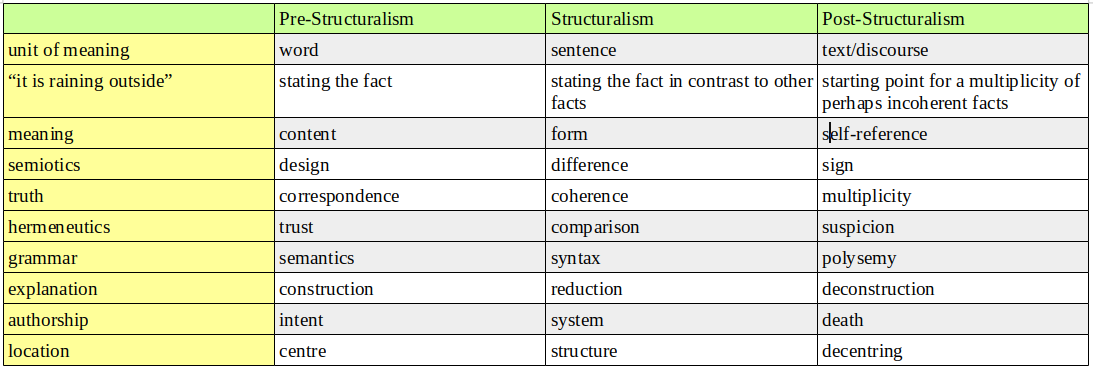
\includegraphics[scale=.3]{./structable.png}
% \end{figure}
% \end{frame}

\begin{frame}
  \frametitle{iClicker Question}
Choose from the following options. This item will not be graded.
\begin{block}{iClicker Question}
Which one of these does NOT belong to the interpreter's credo?
\end{block}
\begin{description}
\item[A\hspace{.2in}$\blacktriangleright$] I believe in hermeneutic realism
\item[B\hspace{.2in}$\blacktriangleright$] I believe in hermeneutic restoration
\item[C\hspace{.2in}$\blacktriangleright$] I believe in hermeneutic responsibility
\item[D\hspace{.2in}$\blacktriangleright$] I believe in hermeneutic rationality
\end{description}
\end{frame}

\begin{frame}
  \frametitle{iClicker Question}
Choose from the following options. This item will not be graded.
\begin{block}{iClicker Question}
Which philosopher is known for the idea of ``deconstruction''?
\end{block}
\begin{description}
\item[A\hspace{.2in}$\blacktriangleright$] Friedrich Nietzsche
\item[B\hspace{.2in}$\blacktriangleright$] Augustine
\item[C\hspace{.2in}$\blacktriangleright$] S{\/o}ren Kierkegaard
\item[D\hspace{.2in}$\blacktriangleright$] Jacques Derrida
\end{description}
\end{frame}

\begin{frame}
  \frametitle{Kierkegaard's Three Parables}
  \begin{itemize}
  \item ``the error of coming to inspect the mirror instead of to see
    oneself in the mirror'' (15) Vanhoozer's double reading
  \item the lover's letter in a strange language: reading vs toiling
    and moiling with a dictionary
  \item the royal ordinance and its interpretations
  \end{itemize}
\end{frame}

\begin{frame}
  \frametitle{Incredulity Towards Meaning}
  Hermogenes (the conventionalist), Cratylus (the postmodernist), and
  Socrates (the Platonist). Vanhoozer wants to sustain Plato's concern
  to defend the possibility of speaking truly. This is a contrast to,
  for example, Joseph Margolis, who maintains that
  \begin{quote}
    {\ldots} what we take to be determinate reality is actually an
    effect of our linguistic practices
  \end{quote}
  for example
  \begin{itemize}
  \item Canada (political practice)
  \item Marriage (social practice)
  \item God (religious practice)
  \end{itemize}
\end{frame}

\begin{frame}
  \frametitle{The Literary Turn in Contemporary Philosophy}
According to Margolis, interpretation produces not commentaries, but
the text (18). There are criteria for interpretation, but they depend
on cultural practice.
\begin{itemize}
\item ``The rise of hermeneutics parallels the fall of epistemology''
  (19).
\item ``With the waxing of texts came the waning of facts'' (20).
\end{itemize}
Hermeneutics, however, undermines itself. Under its rule, philosophy
becomes a branch of literature. The literary nature of Derrida's
writings and Searle's critique from the standpoint of analytic
philosophy. 
\end{frame}

\begin{frame}
  \frametitle{The Literary Turn in Contemporary Philosophy}
  \begin{quote}
    Philosophers typically distinguish their own talk about the world
    from other kinds: for instance, philosophy works with logic and
    seeks literal truth and the light of clear and distinct ideas, while
    literature plays with metaphors and other cloudy figures of
    speech under dark rhetorical skies. Derrida would have none of
    it. (21)
  \end{quote}
  Is language the ``means humans use creatively to colonize a
  meaningless world'' (Nietzsche)?
\end{frame}

\begin{frame}
  \frametitle{Deconstruction}
  A critique of logocentrism (priests and their Word of God;
  philosophers and their Reason/Truth/Meaning).

  \bigskip

  Where is the priority: are questions of power answered within
  framework of truth (``the truth will set you free,'' John 8:32); or
  are questions of truth answered within a framework of power
  (Nietzsche)? (21)
  \begin{quote}
    ``text'' now covers everything from written works to our
    individual histories to reality itself (21)
  \end{quote}
\end{frame}

\begin{frame}
  \frametitle{Three Ages of Criticism}
  \begin{tabular}{|l|l|l|}\hline
        metaphysics       & epistemology                & ethics         \\ \hline 
        author            & text                        & reader         \\ \hline
        realism           & rationality                 & responsibility \\ \hline
        non-realism       & relativism                  & freeplay       \\ \hline
        F. Schleiermacher & new criticism/structuralism & S. Fish        \\ \hline
  \end{tabular}
\end{frame}

\begin{frame}
  \frametitle{The Theological Dimension}
  \begin{quote}
    It is wrong always, everywhere, and for anyone, to believe anything upon insufficient evidence. (W. K. Clifford, 32)
  \end{quote}
  By contrast, the interpreter's credo (31):
  \begin{itemize}
        \item I believe in hermeneutic realism
        \item I believe in hermeneutic rationality
        \item I believe in hermeneutic responsibility
  \end{itemize}
Augustinian hermeneutics: the principle of charity.
\begin{quote}
  The Golden Rule, for hermeneutics and ethics alike, is to treat others---texts, persons, God---with love and respect. (32)
\end{quote}
\end{frame}

\end{document}
